\documentclass[a4paper,10pt]{article}
\usepackage{%
	amsfonts,%
	amsmath,%	
	etex,%
	amssymb,%
	amsthm,%
	babel,%
	bbm,%
	%biblatex,%
	caption,%
	centernot,%
	color,%
	enumerate,%
	epsfig,%
	epstopdf,%
	geometry,%
	graphicx,%
	hyperref,%
	latexsym,%
	mathtools,%
	multicol,%
	pgf,%
	pgfplots,%
	pgfplotstable,%
	pgfpages,%
	proof,%
	psfrag,%
	subfigure,%	
	tikz,%
	ulem,%
	url%
}	

\usepackage[mathscr]{eucal}
\usepgflibrary{shapes}
\usetikzlibrary{%
  arrows,%
	backgrounds,%
	chains,%
	decorations.pathmorphing,% /pgf/decoration/random steps | erste Graphik
	decorations.text,%
	matrix,%
  	positioning,% wg. " of "
  	fit,%
	patterns,%
  	petri,%
	plotmarks,%
  	scopes,%
	shadows,%
  	shapes.misc,% wg. rounded rectangle
  	shapes.arrows,%
	shapes.callouts,%
  	shapes%
}

\theoremstyle{plain}
\newtheorem{thm}{Theorem}[section]
\newtheorem{lem}[thm]{Lemma}
\newtheorem{prop}[thm]{Proposition}
\newtheorem{cor}[thm]{Corollary}

\theoremstyle{definition}
\newtheorem{defn}[thm]{Definition}
\newtheorem{conj}[thm]{Conjecture}
\newtheorem{exmp}[thm]{Example}
\newtheorem{assum}[thm]{Assumptions}
\newtheorem{axiom}[thm]{Axiom}

\theoremstyle{remark}
\newtheorem{rem}{Remark}
\newtheorem{note}{Note}

\newcommand{\norm}[1]{\left\lVert#1\right\rVert}
\newcommand{\indep}{\!\perp\!\!\!\perp}
\DeclarePairedDelimiter\abs{\lvert}{\rvert}%
%\DeclarePairedDelimiter\norm{\lVert}{\rVert}%
\newcommand{\tr}{\operatorname{tr}}
\newcommand{\R}{\mathbb{R}}
\newcommand{\Q}{\mathbb{Q}}
\newcommand{\N}{\mathbb{N}}
\newcommand{\E}{\mathbb{E}}
\newcommand{\Z}{\mathbb{Z}}
\newcommand{\B}{\mathscr{B}}
\newcommand{\C}{\mathcal{C}}
\newcommand{\T}{\mathscr{T}}
\newcommand{\F}{\mathcal{F}}
\newcommand{\G}{\mathcal{G}}
%\newcommand{\ba}{\begin{align*}}
%\newcommand{\ea}{\end{align*}}

\makeatletter
\def\th@plain{%
  \thm@notefont{}% same as heading font
  \itshape % body font
}
\def\th@definition{%
  \thm@notefont{}% same as heading font
  \normalfont % body font
}
\makeatother
\date{}
\title{Lecture 2: Characterizations and Properties of Poisson Process}
\author{Parimal Parag}

\begin{document}
\maketitle

\section{Characterizations of the Poisson Process}

In the previous section, we have shown that Poisson process has stationary, independent increment property. Now, consider any point process with independent stationary increments. From the discussion in the previous section, it follows that the inter-arrival times have to be \emph{iid} with exponential distribution. Such a characterization does not exclude the possibility of more than one arrival at any time instant. Additionally, if we constrain jump sizes to be unity along with stationary independent increments, the process will be a Poisson process. There are stochastic processes which are stationary independent increment and not Poisson. For example, batch/compound Poisson point process and Brownian motion. We have three alternative characterization of the Poisson processes below. 

\begin{defn}[SII and Joint Distribution]\label{defn:SIIJoint} Let $t_0 = 0$, and $\{t_i: 1 \leq i \leq k\}$ be an increasing sequence. A stationary independent increment point process $\{N(t),~t\geqslant 0\}$, such that $N(0) = 0$ is Poisson process if 
%\begin{figure}[h!]
%\center
  %% Requires \usepackage{graphicx}
  %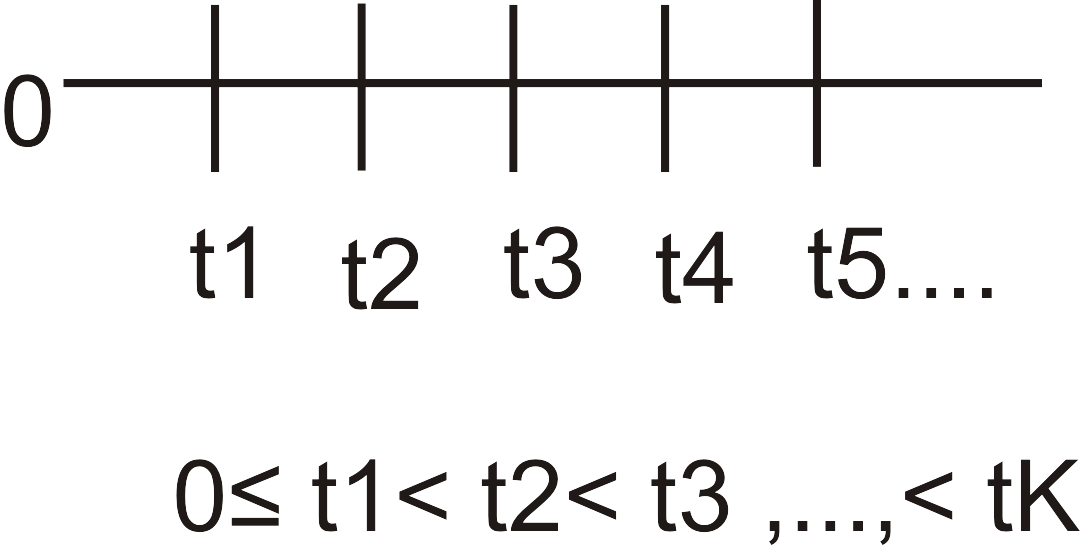
\includegraphics[width=2.8in, height=0.9in]{Figures/SPQT.png}\\
 %% \caption{}\label{}
%\end{figure}
\begin{equation*}
  \Pr\{\bigcap_{i=1}^k \{N(t_i)-N(t_{i-1})= n_{i}\}\} = \prod_{i=1}^{k}\frac{(\lambda(t_{i}-t_{i-1}))^{n_{i}}}{n_{i}!} e^{-\lambda (t_{i}-t_{i-1})}.
\end{equation*}
\end{defn}

\begin{defn}[SII and Marginal Distribution]\label{defn:SIIMarginal} A point process $\{N(t),~t\geqslant 0\}$ is said to be Poisson process with rate $\lambda$ if it has stationary independent increments, and 
\begin{equation*}
\Pr\{N(t)=n\}= \frac{(\lambda t)^{n}}{n!} e^{-\lambda t}, n\in \mathbb{Z}^+.
\end{equation*}
\end{defn}

\begin{defn}[SII and Infinitesimal Arrivals]\label{defn:SIIInfinitesimal} A point process $\{N(t),~t\geqslant 0\}$ is said to be Poisson process with rate $\lambda$ if it has stationary independent increments, and 
\begin{eqnarray*}\label{eqn1}
\Pr\{N(t)=0\} &=& 1-\lambda t + o(t), \\
  \Pr\{N(t)=1\} &=& \lambda t + o(t), \\
  \Pr\{N(t)>1\} &=& o(t).
\end{eqnarray*}
\end{defn}

\begin{thm}[Equivalent Characterizations] Definitions~\ref{defn:SIIJoint},~\ref{defn:SIIMarginal},~\ref{defn:SIIInfinitesimal} are equivalent to definition of Poisson process.
\end{thm}
\begin{proof}
We have already shown that Poisson process satisfies the conditions in Definitions~\ref{defn:SIIJoint},~\ref{defn:SIIMarginal}. That is, Definition~\ref{defn:SIIJoint} follows from original definition of Poisson process. It is easy to see that Definition~\ref{defn:SIIMarginal} follows trivially from Definition~\ref{defn:SIIJoint}. It is easy to see that Definition~\ref{defn:SIIMarginal} implies Definition~\ref{defn:SIIInfinitesimal}. We will show that Definition~\ref{defn:SIIInfinitesimal} implies original definition of Poisson process. Hence, we would have shown equivalence of all characterizations.
%will now that 
%We first show that Poisson process satisfy the above set of equations. We have shown that the Poisson process has stationary, independent increment property  and 
%\begin{equation*}
  %\Pr\{N(t)= n\} =  e^{-\lambda t} \frac{(\lambda t)^{n}}{n!}, n\in \mathbb{Z}^+.
%\end{equation*}
  %\begin{eqnarray*}
  %\Pr\{N(t)=0\} &=& e^{-\lambda t} = 1-\lambda t + o(t).\\
   %\Pr\{N(t)=1\}&=& e^-\lambda t (\lambda t) \\
  %&=& e^-\lambda t^{(1-e^-\lambda t+ o(t))}\\
   %&=& \lambda t- \lambda^{2} t^{2}+ o(t) \lambda t.
   %\end{eqnarray*}
   %Since $\frac{\lambda^{2} t^{2}}{t} =  \lambda^{2} t$ and $\lim _{t\downarrow 0}\lambda^{2} t= 0$, $\lambda^{2} t^{2} =o(t)$. Consider  $\lambda t o(t) = 0$.   $\lim _{t\downarrow 0}\frac{\lambda t o(t)}{t} = \lambda \lim _{t\downarrow 0} o(t)$. Since sum of two $o(t)$ terms is again an $o(t)$ term, $\Pr\{N(t)=1]= \lambda t + o(t)$. Since the three probability terms given should sum up to 1, $ \Pr\{N(t)>1]=o(t)$. So, we showed that the  Poisson Process has the above stated property. 	Now, we show the converse. 
	
To show the converse, it suffices to show that the time to first jump $X_{1}$ is exponentially distributed with rate $\lambda$. To this end, let $f(t) = \Pr\{X_{1}>t\}$ for $t \geq 0$. It is clear that for any arbitrary $s>0$, we have
\begin{equation*}
\{X_{1}>t+s\}\iff \{N(t)=0\}\cap\{N(t+s)-N(t)=0\}.
\end{equation*}
Due to independent increment property of $N(t)$, we know that $N(t)$ and $N(t+s)-N(t)$ are independent. Further, due to stationarity of the increments, $N(t+s) - N(t)$ has same distribution as $N(s)$. Therefore, we can write
\begin{equation*}
 f(t+s) =   \Pr\{X_{1}>t+s\} = \Pr\{X_{1}>t\} \Pr\{X_{1}>s\} = f(s)f(t).
\end{equation*}
Since, $f$ is right continuous non-negative function with such a property, $f(t) = \exp(-\alpha t)$ for some $\alpha > 0$ and all $t \geq 0$, from last lecture. Since, $1 - f(0) = \lambda t + o(t)$, we conclude that $\alpha = \lambda$.
%\begin{eqnarray*}
   %&=& f(t) \Pr\{N(s)=0\} \\
   %&=& [1- \lambda s + o(s)] f(t) \\
  %f(t+s) &=& [1- \lambda s + o(s)] f(t)\\
  %\frac{f(t+s)-f(t)}{s} &=& \frac{o(s)}{s}f(t)- \lambda f(t) \\
  %\lim_{s\downarrow0}  \frac{f(t+s)-f(t)}{s}  &=& f(t) \times 0 - \lambda f(t) = -\lambda f(t) \\
 %f'(t) &=& - \lambda f(t), t\geq 0.
%\end{eqnarray*}
%where (a) follows from independent increment property and (b) follows from stationary increment property.We have shown that $f$ has a derivative and is equal to $-\lambda f(t)$.\\
%\begin{eqnarray*}
%% \nonumber to remove numbering (before each equation)
   %\Pr\{N(t)=0\} &=& 1- \lambda (t)+ 0(t) \\
  %\lim _{t\downarrow0}\Pr\{N(t)=0\} &=& 1 \\
  %1= \lim _{t\downarrow0}\Pr\{N(t)=0\}&=& \lim _{t\downarrow0}\Pr\{X_{1}>t\}\\
   %&=& \Pr\{X_{1}>0]  \\
  %\therefore f(0) &=& 1
  %\end{eqnarray*}
  %Solve $\frac{df(t)}{dt} = -\lambda f(t), ~t\geq 0$, $f(0)= 1$. We get $f(t) = e^{-\lambda t}$.
   %\begin{eqnarray*}
  %\therefore f(t) &=&  \Pr\{X_{1}>t\}= e^{-\lambda t}.\\
  %X_{1}&\sim & exp (\lambda ).
%\end{eqnarray*}

%We next show that first two inter-arrival times $X_{1}, X_{2}$ are independent. To this end, note that 
%\begin{equation*}
%\{X_1 = t_1, X_2 = t_2\} \iff \{N(t_1)=1\}\cap\{N(t_2+t_1)-N(t_1)=1\}.
%\end{equation*}
%From stationary independent increment property of $N(t)$, we get  
%\begin{eqnarray*}
 %P(X_{1}=t_{1}, X_{2}=t_{2}) && t_{1} >0, t_{2}>0\\
  %P(X_{1}=t_{1})P (X_{2}=t_{2}| X_{1}=t_{1})&=& \lambda e^{-\lambda t_{1}} \\
   %&=& \lambda e^{-\lambda t_{1}} \Pr\{N_{t_{1}+t_{2}}-\delta=1,N_{t_{1}+t_{2}}=2|N(t_{1})=1) \\
   %&=& \lambda e^{-\lambda t_{1}} \Pr\{Nt_{2}=1] \\
   %&=& \lambda e^{-\lambda t_{1}} \lambda e^{-\lambda t_{2}}  \\
   %X_{1} \perp X_{2}&and & X_{1}, X_{2} \sim exp (\lambda).
%\end{eqnarray*}
%Proof follows from induction
\end{proof}

We study these characterizations because Poisson process is a fundamental process, just like Gaussian process among the class of distributions.

\subsection{Non-Homogeneous Poisson Process}
From the characterization of Poisson process just stated, we can generalize to non-homogeneous Poisson process. In this case, the rate of Poisson process $\lambda$ is time varying. It is not clear from the first two characterizations, how to generalize the definition of Poisson process to the non-homogeneous case. We used third characterization of Poisson process for this generalization. 

\begin{defn}[Non-Homogeneous Poisson Process]\label{defn:NonHomogeneousPoisson} A point process $\{N(t),~t\geqslant 0\}$ is said to be \textbf{non-homogeneous Poisson process} with instantaneous rate $m(t)$ if it has stationary independent increments, and 
 \begin{eqnarray*}\label{eq:NonHomogeneousPoisson}
 \Pr\{N(t)=0\}&=&1-m(t)+o(t). \\
  \Pr\{N_{t+\delta}-N(t)=0\} &=& 1-m(t)\delta+o(\delta). \\
   \Pr\{N_{t+\delta}-N(t)=1\} &=& m(t)\delta+o(\delta). \\
   \Pr\{N_{t+\delta}-N(t)>1\} &=& o(\delta). \\
   \end{eqnarray*}
\end{defn}

\begin{prop}[Non-Homogeneous Distribution] Distribution of non-homogeneous Poisson process $N(t)$ with instantaneous rate $m(t)$ is given by
 \begin{equation*}
 \Pr\{N(t)=n\}=\frac{(\bar{m}(t))^n}{n!}e^{-\bar{m}(t)},
 \end{equation*}
where $\bar{m}(t)$ is the cumulative rate till time $t$, i.e. $\bar{m}(t)=\int_{0}^{t}m(s)ds$. 
\end{prop}
\begin{proof}
Let's denote $f(t) = \Pr\{N(t)=0\}$. Further, from independent increment property of $N(t)$, we notice that $\{N(t+\delta) = 0\}$ is intersection of two independent events given below, 
\begin{equation*}
\{N(t+\delta)=0\} \iff \{N(t)=0\}\cap\{N(t+\delta)-N(t)=0\}.
\end{equation*}
From Definition~\ref{defn:NonHomogeneousPoisson}, it follows that
\begin{equation*}
 f(t+\delta) = f(t)[1 - m(t) + o(\delta)].
\end{equation*}
Re-arranging the terms in the above equation, dividing by $\delta$, and taking limit as $\delta \downarrow 0$, we get 
\begin{equation*}
f'(t) = -m(t)f(t).
\end{equation*}
Since $f(0) = 1$, it can be verified that $f(t) = \exp(-\bar{m}(t))$ is solution for $f(t)$.

%\begin{eqnarray*}
  %f(t+\triangle) &=& \Pr\{N_{t+\triangle}=0] \\
   %&=&  \Pr\{N(t)=0, N_{t+\triangle}-N(t)=0]\\
   %&\stackrel{(a)}{=}& \Pr\{N(t)=0] \Pr\{N_{t+\triangle}-N(t)=0]\\
   %&=& f(t)[1-m(t)\triangle +o(\triangle)].\\
%\frac{f(t+\triangle)-f(t)}{\triangle} &=& -m(t) f(t) +f(t) \frac{0(\triangle)}{\triangle}. \\
  %\lim_{\triangle\downarrow 0}\frac{f(t+\triangle)-f(t)}{\triangle} &=& -m(t) f(t) \\
 %\frac{d f(t)}{t} &=& -m(t) f(t),  \\
 %\end{eqnarray*}
 %where (a) follows from independent increment property. Since, $\overline{m}(t)=\int ^{t}_{0} m(s) ds $, $f(t)=\Pr\{N(t)=0]$, $ f(0)=\Pr\{N_{0}=0] =1$ the solution of the differential equation can be verified to be $f(t)=e^{-\overline{m}(t)}$, as follows: 
 %\begin{eqnarray*}
     %f(0)&=& e^{-\overline{m}(t)}\\
  %&=& e^{-0}=1 \\
  %f'(t) &=& e^{-\overline{m}(t)}\frac{d}{dt} \int^{t}_{0}m(S) ds\\
  %&=& m(t)e^{-\overline{m}(t)}, t\geqslant 0 \\
  %\end{eqnarray*}
  %
  %\begin{eqnarray*}
  %\Pr\{N_{t+\triangle}-N(t)=0] &=& 1-m(t)\triangle +o(\triangle) \\
  %\Pr\{N_{\triangle}-N_{0}=0] &=& 1-m(0)\triangle +o(\triangle) 
  %\end{eqnarray*}
  %Since $ N_{0}=0$, 
  %\begin{eqnarray*}
   %\Pr\{N_{\triangle} =0]&=& 1-m(0)\triangle +0(\triangle) \\
  %\lim_{\triangle\downarrow 0}f(\triangle) &=& f(0)=1.
%\end{eqnarray*}
We have shown $\Pr\{N(t)=0\} = \exp(-\bar{m}(t))$. By induction, we can show the result for any $n$.
\end{proof}

\subsection{Properties of Poisson Process}

\begin{prop}[Conditional Distribution of First Arrival Instant] For a Poisson process $\{N(t), t\geqslant 0\}$, distribution of first arrival instant $S_1$ conditioned on $\{N(t)=1\}$ is uniform between $[0,t)$.
\end{prop}
\begin{proof} Since $N(t) = 1$, we know that conditional distribution of $S_1$ is supported on $[0,t)$. Further, for any $0 \leq u < t$, we can write $\{S_1 = u, N(t) = 1\}$ as intersection of two independent events, as follows
\begin{equation*}
\{S_1 = u, N(t) = 1\} \iff \{S_1 = u\}\cap\{X_2 > t - u\}.
\end{equation*}
Therefore, integrating LHS with respect to $u$ in interval $[0,s]$ for $s < t$, we obtain
\begin{equation*}
\Pr\{S_1 \leq s, N(t) = 1\} = \int_{0}^{s}du \lambda \exp(-\lambda u)\exp(-\lambda (t-u)) = s\lambda\exp(-\lambda t).
\end{equation*}
Since $\Pr\{N(t) = 1\} = \lambda t \exp(-\lambda t)$, it follows that 
\begin{equation*}
\Pr\{S_1 \leq s| N(t) = 1\} = \begin{cases}\frac{s}{t}, & s < t\\ 0, & s \geq t.\end{cases}.
\end{equation*}
%\noindent For the  with rate $0<\lambda< \infty$, we would like to find the density.
%\begin{eqnarray*}
%% \nonumber to remove numbering (before each equation)
  %P(S_{1}\mid N(t)=1), t>0 \\
  %P_{S_1}(S \mid N(t)=1) \\
  %P(s\leq S_{1} \leq s+h \mid N(t)=1)\\
   %&\approx& h P_{S_1}(S \mid N(t)=1 \\
  %P(s\leq S_{1}< s+h \mid N(t)=1)\\
   %&=& \frac{P(s\leq S_{1}< s+h,N(t)=1)}{P(N(t)=1)}\\
   %&=& \frac{\Pr\{s\leq S_{1}<s+h,X_{2}>t-(s+h))}{\lambda t e^{-\lambda t}} \\
   %&=& \frac{h \lambda e^{-\lambda h} e^{-\lambda (t-(s+h))}}{h{\lambda t} e^{-\lambda t}}.
   %\end{eqnarray*}
   %Take  $\lim _{h\rightarrow 0}\frac{1}{t}{e^{-\lambda h}} =\frac{1}{t}.$ Thus, the conditional density is the density of a uniform random variable distributed over the interval $[0,t].$ 
\end{proof}

This property of Poisson process can be generalized for any set of arrival instants.
\begin{prop}[Conditional Distribution of Arrival Instants] For a Poisson process $\{N(t), t\geqslant 0\}$, joint distribution of arrival instant $\{S_1, \ldots, S_n\}$ conditioned on $\{N(t)=n\}$ is identical to joint distribution of order statistics of $n$ \emph{iid} uniformly distributed random variables between $[0,t]$.
\end{prop}
\begin{proof} Let $\{ 0 \leq s_i \leq t: 1 \leqslant i \leqslant n\}$ be a sequence of non-negative increasing numbers between $0$ and $t$. If we denote $s_{-1} = 0$, then we can write 
\begin{equation*}
\bigcap_{i=1}^n\{S_i = s_i\}\cap\{N(t) = n\} \iff \bigcap_{i=1}^n\{X_i = s_i - s_{i-1}\}\cap\{X_{n+1} > t - s_n\}.
\end{equation*}
Note that all the events on RHS are independent events. Therefore, it is easy to compute the joint distribution of $\{S_1,\ldots, S_n\}$, as 
\begin{align*}
\Pr\bigcap_{i=1}^n\{S_i \leq s_i\}\cap\{N(t) = n\} &= \int_{0}^{s_1}du_1\cdots\int_{0}^{s_n}du_n \prod_{i=1}^n\lambda \exp(-\lambda (u_i-u_{i-1})\exp(-\lambda (t-u_n))\\
&= \lambda^n\exp(-\lambda t)\prod_{i=1}^ns_i.
\end{align*}
Since $\Pr\{N(t) = n\} = \exp(-\lambda t)(\lambda t)^n/n! $, it follows that 
\begin{equation*}
\Pr\{S_1 \leq s_1,\ldots, S_n\leq s_n | N(t) = n\} = 
\begin{cases}
n!\prod_{i=1}^n\frac{s_i}{t} & s < t\\ 
0 & s \geq t.
\end{cases}
\end{equation*}
%\begin{eqnarray*}
%% \nonumber to remove numbering (before each equation)
    %&\Pr\{s_{1}\leq S_{1}<s_{1}+h, s_{2}\leq S_{2}<s_{2}+h, ...s_{n}\leq S_{n}\leq s_{n}+h \mid N(t)=n]  \\
   %&=   \frac{\Pr\{s_{1}\leq S_{1}<s_{1}+h, s_{2}\leq S_{2}<s_{2}+h,...,s_{n}\leq S_{n}\leq s_{n}+h,N(t)=n]}{\Pr\{N(t)=n]} \\
   %&=  \frac{\Pr\{s_{1} \leq S_{1}<s_{1}+h_{1},s_{2}-s_{1}\leq X_{2}<s_{2}- (s_{1}+h),..., X_{n+1}> t-s_{n}]}{\Pr\{N(t)=n]} \\
   %&\stackrel{(a)}{=}  \frac{\Pr\{s_{1 \leq S_{1}<s_{1}+h}]\Pr\{s_{2}-s_{1}\leq X_{2}<s_{2}-s_{1}+h] \Pr\{X_{n+1}>t -s_{n}]}{\Pr\{N(t)=n]}\\
   %&=  \frac{\lambda h e^{-s_{1}\lambda}h \lambda e^{-(s_{2}-s_{1})\lambda},..., e^{-(t-s_{n})\lambda}}{(\lambda t)^{n}\frac{e^{-\lambda t}}{n!}} 
   %\end{eqnarray*}
   %\begin{eqnarray*}
    %\lim _{h\rightarrow 0} \frac{ \lambda h e^{-s_{1}\lambda}h \lambda e^{-(s_{2}-s_{1})\lambda},... e^{-(t-s_{n})\lambda}}{h^{n}(\lambda t)^{n}\frac{e^{-\lambda t}}{n!}}=\frac{n!}{t^{n}}.
%\end{eqnarray*}
%where (a) follows as $X_i$s are independent. 
Let $U_{1},\ldots,U_{n}$ are \emph{iid} Uniform random variables in $[0,t]$. Then, conditioned on $\{N(t)=n\}$, the $n$ arrival instants have the same joint distribution as the order statistics  of $U_1 \ldots, U_n$.
\end{proof}

We give some more properties of the Poisson process.
\begin{thm}[Sum of Independent Poissons] Let ${N_1(t), t \geqslant  0}$ and ${N_2(t), t \geqslant  0}$ be two independent Poisson processes with rats $\lambda_{1}$ and $\lambda_{2}$ respectively. Then, the process $N(t)= N_{1}(t) +N_{2}(t)$ is Poisson with rate $\lambda_{1}+\lambda_{2}$.
\end{thm}
\begin{proof} We need to show that $\{N(t)\}$ has stationary independent increments, and 
\begin{equation*}
	\Pr\{N(t)=n\}=   \exp(-(\lambda_{1}+\lambda_{2})t)\frac{(\lambda_{1}+\lambda_{2})^n t^n}{n!}.
\end{equation*}
For two disjoint interval $(t_{1}, t_{2})$ and $(t_3,t_4)$, we can see that for both processes $N_{1}(t)$ and $N_2(t)$,  arrivals in $(t_{1}, t_{2})$ and $(t_3,t_{4})$ are independent. Therefore, $N(t)$ has independent increment property. Similarly, we can argue about the stationary increment property of $\{N(t)\}$. Further, we can write 
\begin{equation*}
	\{N(t)=n\} = \bigcup_{k=0}^n\{\{N_1(t) = k\}\cap\{N_2(t) = n-k\}\}.
\end{equation*}
Since $N_1(t)$ and $N_2(t)$ are independent, we can write
\begin{align*}
	\Pr\{N(t)=n\} &= \sum_{k=0}^n\exp(-\lambda_1t)\frac{(\lambda_1t)^k}{k!}\exp(-\lambda_2t)\frac{(\lambda_2t)^{n-k}}{(n-k)!},\\
	&= \frac{\exp(-(\lambda_1+\lambda_2)t)}{n!}\sum_{k=0}^n\binom{n}{k}(\lambda_1t)^k(\lambda_2t)^{n-k}.% = \exp(-(\lambda_1+\lambda_2)t)\frac{\{(\lambda_1+\lambda_2)t\}^n}{n!}.
\end{align*}
Result follows by recognizing that summand is just binomial expansion of $[(\lambda_1 + \lambda_2)t]^n$.
%\begin{eqnarray*}
%% \nonumber to remove numbering (before each equation)
  %\Pr\{N(t)=n] &=& \Pr\{N_{1}(t)+ N_{2}(t)= n] \\
   %&=& \sum_{n1} P [N_{1}(t)=n_{1},N_{2}(t)= n-n_{1} ] \\
  %&=& \sum_{n_{1}}\frac{e^{-\lambda _{1}t}(\lambda_{1}t)^{n_{1}}}{n_{1}!}e^{-\lambda_{2}t}\frac{(\lambda_{2}t)^{(n-n_{1})}}{(n-n_{1})!} \\
   %&=&\sum_{n_{1} (\lambda _{2}t)} \frac{e^{-(\lambda_{1}+\lambda_{2})t} (\lambda_{1}t)^{n1}(\lambda_{2}t)^{-n_{1}}}{n_{1}! (n-n_{1})!} \\
   %&=& \frac{e^{-(\lambda_{1}+\lambda_{2})t}}{n!}\sum^{n}_{n_{1=0}}\left(\frac{\lambda_{1}}{\lambda_{2}}\right)^{n_{1}}\left(\frac{\lambda_{2}}{n_{1}!}\right)^{n}\frac{n!}{(n-n_{1})!} \\
   %&=&  \frac{e^{-(\lambda_{1}+\lambda_{2})t}}{n!}(\lambda_{1}+\lambda_{2})^{n}t^{n}
%\end{eqnarray*}
\end{proof}
\begin{rem}If independence condition is removed, the statement is not true.
\end{rem}
%\begin{figure}
%\centering
  %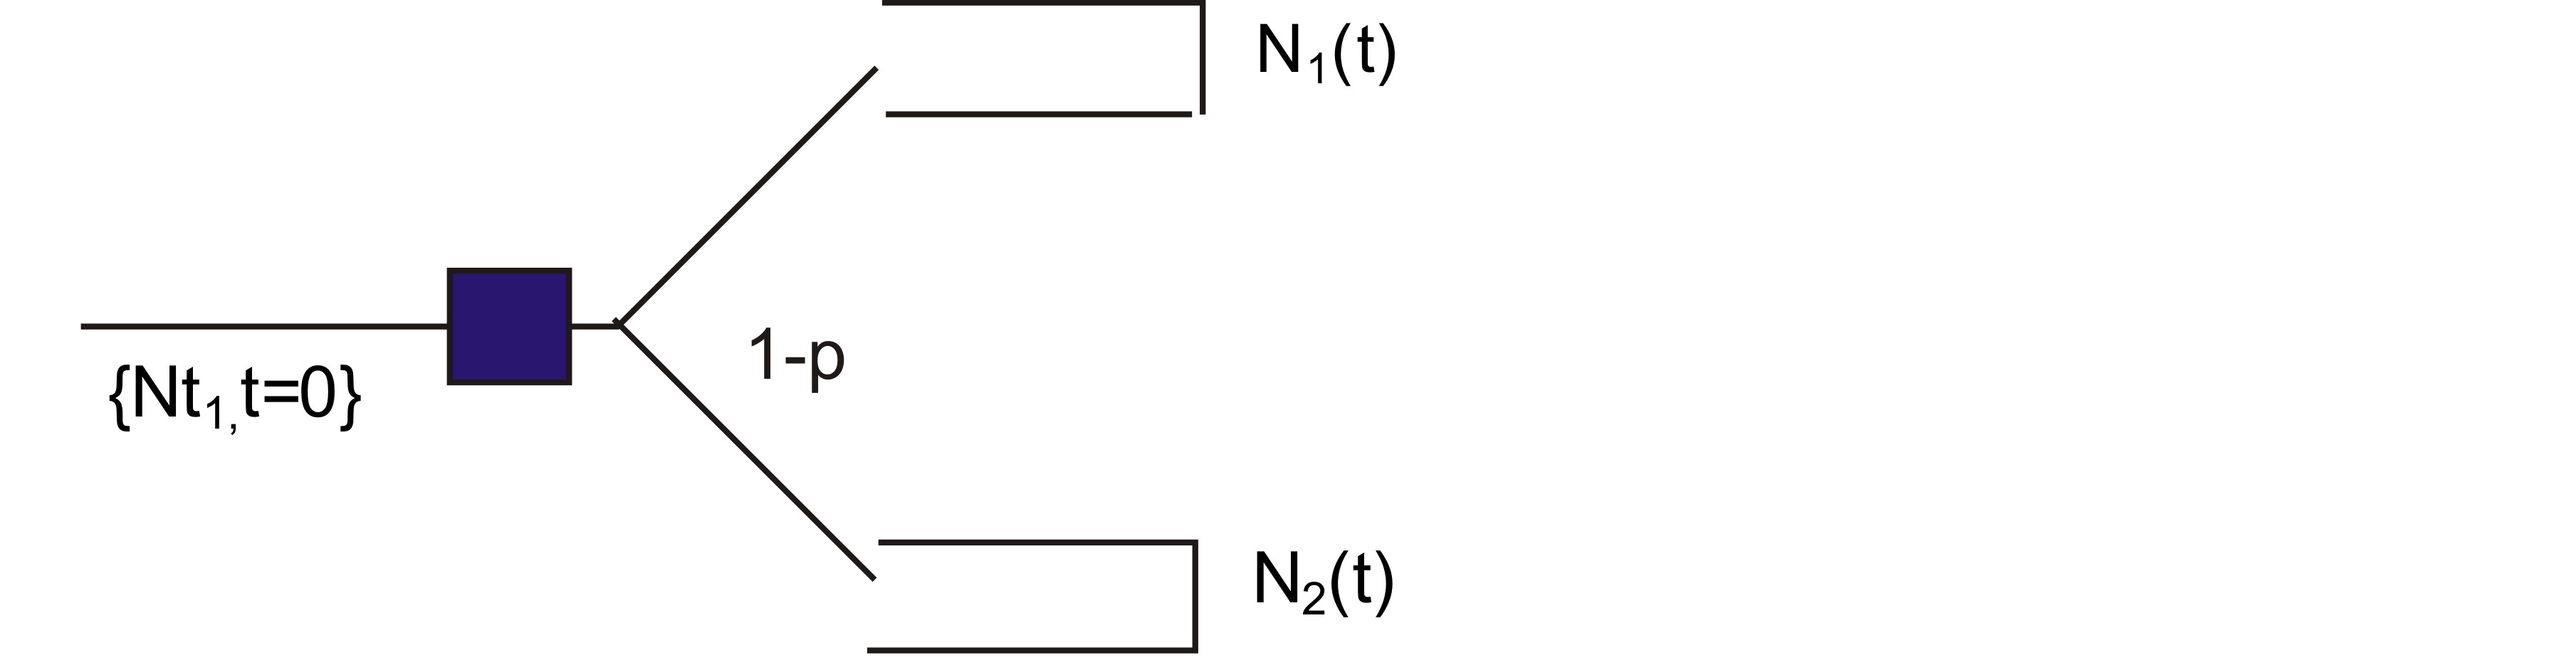
\includegraphics[width=5.0in]{Figures/comment.PNG}\\
 %% \caption{}\label{}
%\end{figure}
\begin{figure}[hhhh]
\center
  \begin{tikzpicture}
[node distance=1cm, draw=black, thick, >=stealth',
axes/.style=,
block/.style={rectangle, draw=black, rounded corners, inner sep=1pt, minimum height=0.8cm, minimum width=0.5cm},
queue/.style={rectangle, draw=white, rounded corners, inner sep=1pt, minimum height=0.8cm, minimum width=0.5cm}]

\node[block](Nt) at (2,10) {Splitter} 
	edge node[near start,above]{$N(t)$} (0,10);
\node[queue](N1t) [above right=of Nt,xshift=3cm] {}
	edge
	node[near end, above]{$p$}
	node[near start, above]{$N_1(t)$}
	(Nt);
\node[queue](N2t) [below right=of Nt,xshift=3cm] {}
	edge
	node[near end, below]{$1-p$}
	node[near start, above]{$N_2(t)$}
	(Nt);
\begin{scope}[axes]
\draw[->] (0,0) -- (9.5,0) node[right] {$t$} coordinate (time);
\draw[->] (0,0) -- (0,7) node[above] {$N(t)$} coordinate (number of  events);
\foreach \x/\xtext in {0.5/S_{n-3}, 1.5/S_{n-2}, 2.2/S_{n-1},3.2/S_{n}, 5.1/S_{n+1}, 6/S_{n+2}}
	\draw[xshift=\x cm] (0pt,1pt) -- (0pt,-1pt) node[below,fill=white] {$\xtext$};
\foreach \y/\ytext in {1/n-3,2/n-2, 3/n-1, 4/n,5/n+1,6/n+2}
	\draw[yshift=\y cm] (1pt,0pt) -- (-1pt,0pt) node[left,fill=white] {$\ytext$};
\end{scope}
\draw[] (0,0)--(.5,0)--(.5,1)--(1.5,1)--(1.5,2)--(2.2,2)--(2.2,3)--(3.2,3)--(3.2,4)--(5.1,4)--(5.1,5)--(6,5)--(6,6)--(9,6)node[right]{$N(t)$};
\draw[red] (0,0)--(.5,0)--(.5,1)--(3.2,1)--(3.2,2)--(9,2)node[right]{$N_1(t)$};
\draw[blue] (0,0)--(1.5,0)--(1.5,1)--(2.2,1)--(2.2,2)--(5.1,2)--(5.1,3)--(6,3)--(6,4)--(9,4) node[right]{$N_2(t)$};

\end{tikzpicture}

 \caption{Splitting a Poisson process into two independent Poisson processes.}
\label{Fig:IndependentSplitting}
\end{figure}

\begin{thm}[Independent Spilitting] Let $\{N(t), t \geqslant 0\}$ be a Poisson arrival process. Each arrival can be randomly assigned to either arrival type 1 or 2, with probability $p$ and $(1-p)$ respectively, independent of previous assignments. Arrival processes of type 1 and 2 are denoted by $N_1(t)$ and $N_2(t)$ respectively. Then, $\{N_{1}(t), t \geqslant 0\}$,and $\{N_{2}(t), t \geqslant 0\}$ are mutually independent Poisson processes with rates $\lambda p$ and $\lambda (1-p)$ respectively.  
\end{thm}
\begin{proof} To show that ${N_{1}(t), t \geq 0}$ is a Poisson process with rate $\lambda p$, we show that it is stationary independent increment process with the distribution
\begin{equation*}
 \Pr\{N_{1}(t)= n\}  = \frac{(p \lambda t)^{n}}{n!}e^{-\lambda p t}.
\end{equation*}
%\begin{figure}
%\center
  %% Requires \usepackage{graphicx}
  %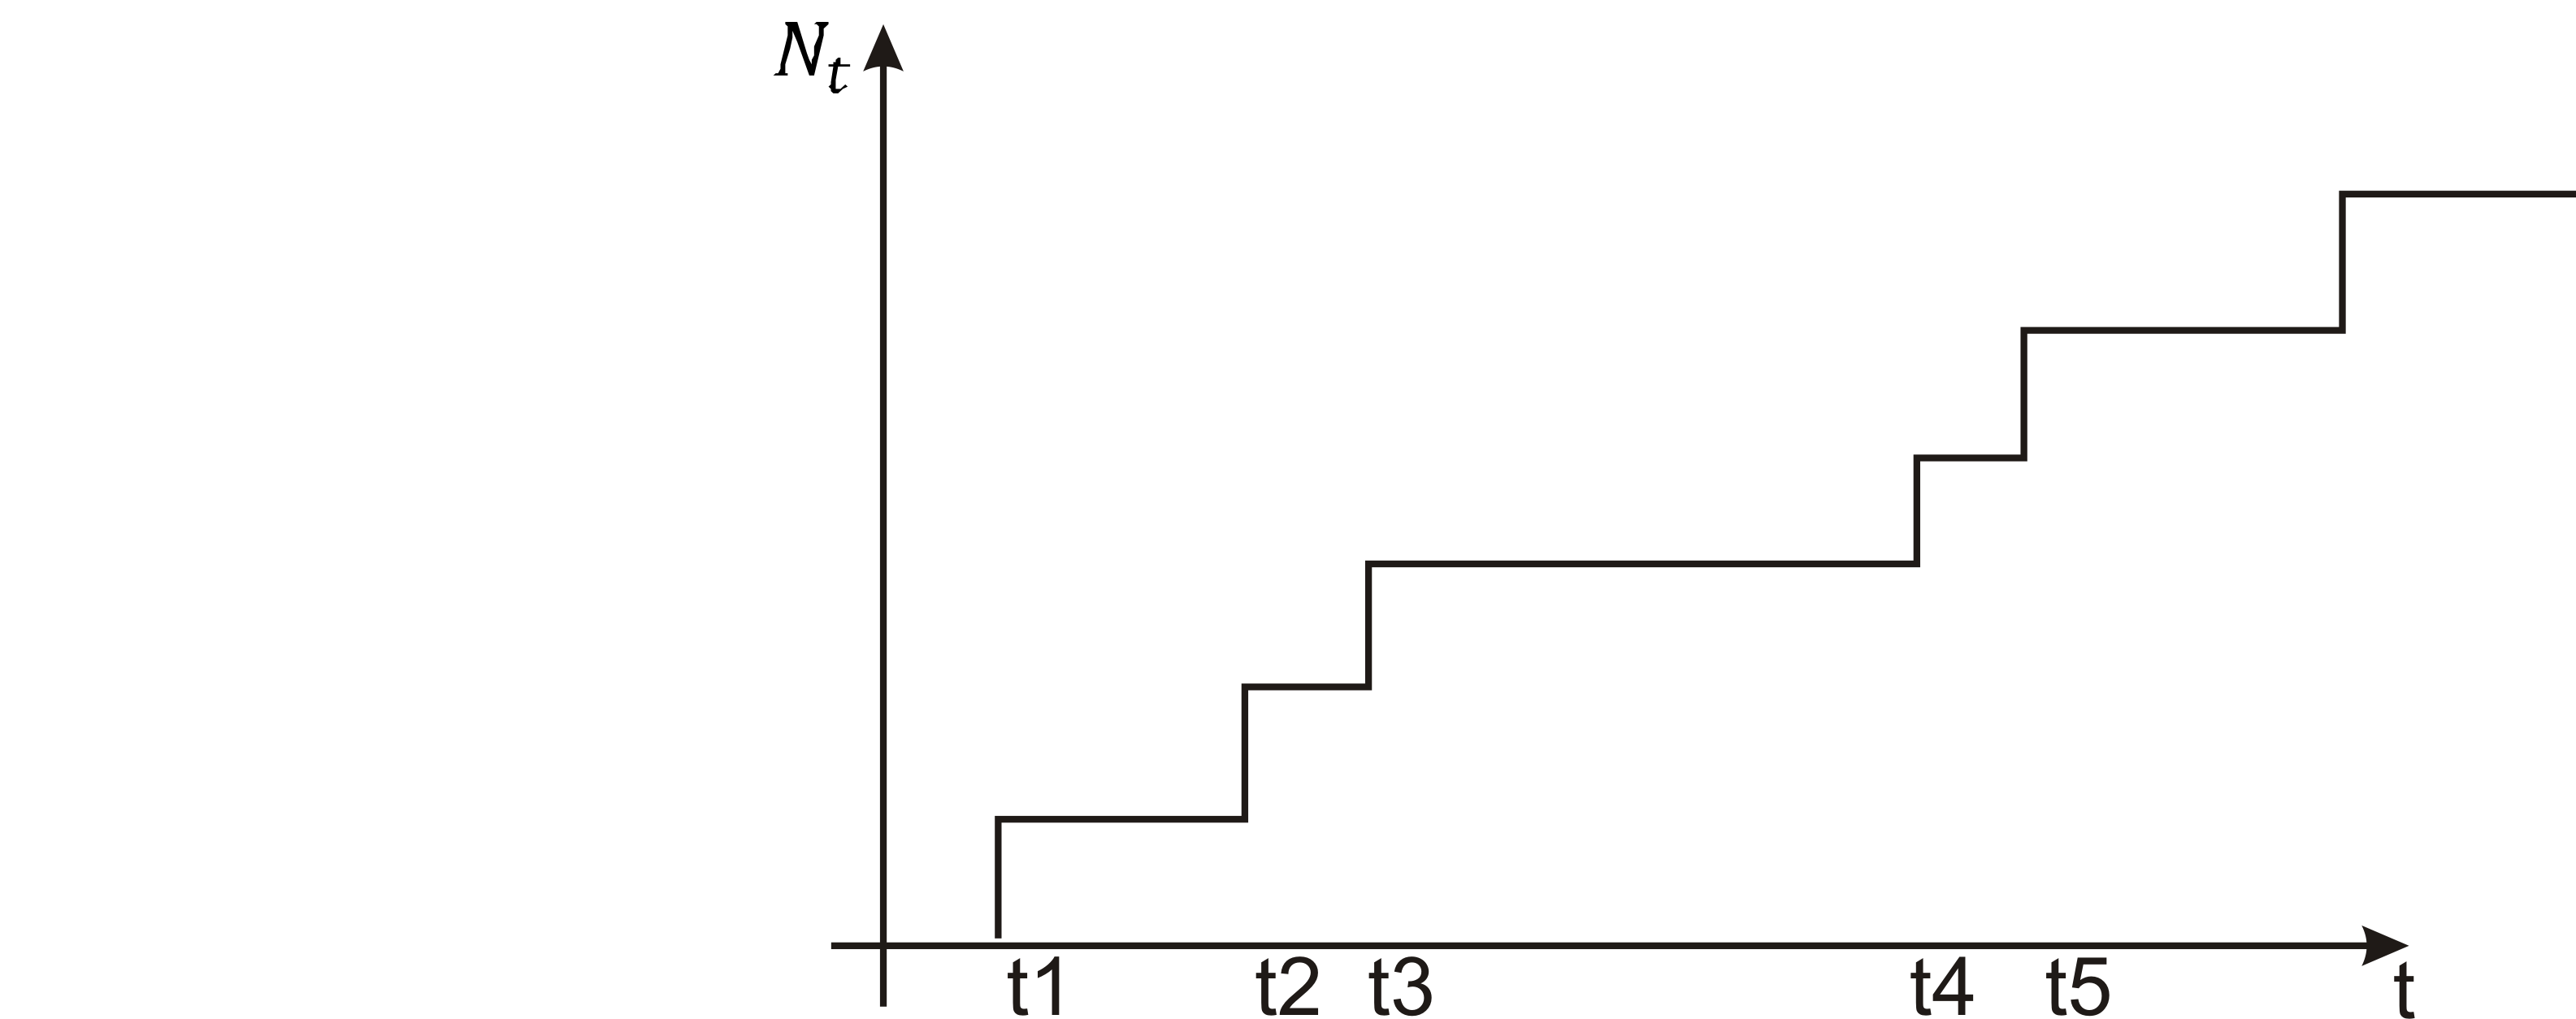
\includegraphics[width=4.5in]{Figures/distr.PNG}\\
 %% \caption{}\label{}
%\end{figure}
The stationary, independent increment property of the probabilistically filtered processes $\{N_1(t), t \geqslant 0\}$ and $\{N_2(t), t \geqslant 0\}$ can be understood and argued out from the example given in the figure. Notice that 
\begin{equation*}
	\{N_1(t)=k\} = \bigcup_{n=k}^\infty\{N(t) = n, N_1(t) = k\}.
\end{equation*}
Further notice that conditioned on $\{N(t) = n\}$, probability of event $\{N_1(t) = k\}$ is merely probability of selecting $k$ arrivals out of $n$, each with independent probability $p$. Therefore, 
\begin{align*}
	\Pr\{N_1(t)=k\} &= \exp(-\lambda t)\sum_{n=k}^\infty\frac{(\lambda t)^n}{n!}\binom{n}{k}p^k(1-p)^{n-k},\\
	&= \exp(-\lambda t)\frac{(\lambda p t)^k}{k!}\sum_{n=k}^\infty\frac{(\lambda(1-p)t)^{n-k}}{(n-k)!}.% = \exp(-p\lambda t)\frac{(p\lambda t)^k}{k!}.
\end{align*}
Recognizing that infinite sum in RHS adds up $\exp(\lambda(1-p)t)$, the result follows. We can find the distribution of $N_2(t)$ by similar arguments. We will show that events $\{N_1(t) = n_1\}$ and $\{N_2(t) = n_2\}$ are independent. To this end, we see that 
\begin{equation*}
	\{N_1(t) = n_1, N_2(t) = n_2\} = \{N(t) = n_1 + n_2, N_1(t) = n_1\}.
\end{equation*}
Using their distribution for $N_1(t), N_2(t)$, and conditional distribution of $N_1(t)$ on $N(t)$, we can show that
\begin{align*}
	\Pr\{N_1(t) = n_1, N_2(t) = n_2\} &= \exp(-\lambda t)\frac{(\lambda t)^{n_1 + n_2}}{(n_1 + n_2)!}\binom{n_1 + n_2}{n_1}p^{n_1}(1-p)^{n_2},\\
	&= \Pr\{N_1(t) = n_1\}\Pr\{N_2(t) = n_2\} .
\end{align*}


  %\begin{eqnarray*}
  %% \nonumber to remove numbering (before each equation)
    %\Pr\{N_{1}(t) =n]&=& \sum^{\infty}_{m=0}\Pr\{N(t)=m, N_{1}(t) = n]  \\
   %&=& \sum^{\infty}_{m=n}\Pr\{N(t)=m] p^{n}(i-p)^{m-n}mC_n\\
   %&=&  \sum^{\infty}_{m=n}\frac{e^{-\lambda t(\lambda t)^{m}}}{m!}p^{n}(1-p)^{m-n}(mC_n)\\
     %&=& e^{-\lambda t}p^{n}\sum_{m=n}\frac{(\lambda t)^{m-n}}{m!}\frac{(1-p)^{m-n}m!}{n!(m-n)!} \\
     %&=& \frac{e^{-\lambda t p}(p \lambda t)^{n}}{n!} \sum^{\infty}_{m=n}e^{-\lambda (1-p)t}\frac{(\lambda (1-p)t)^{m-n}}{(m-n)!} \\
     %&=&  \frac{e^{-\lambda t p}(p \lambda t)^{n}}{n!} \sum^{\infty}_{k=0}e^{-\lambda (1-p)t}\frac{(\lambda (1-p)t)^{k}}{k!}  \\
     %&=& \frac{e^{-\lambda p t}(p \lambda t)^{n}}{n!}.
  %\end{eqnarray*}
%To show that 
%\begin{eqnarray*}
%% \nonumber to remove numbering (before each equation)
   %\{N_{1}(t), t \geq 0\}&\perp&\{N_{2}(t), t \geq 0\}  \\
   %\Pr\{N_{1}(t)&=&n_{1}, N_{2}(t) = n_{2}]\\
    %\Pr\{N(t) = n_{1}+ n_{2}]&=& \frac{e^{-\lambda t} (\lambda t)^{n_{1}+n_{2}}}{(n_{1}+n_{2})!} \\
   %&=&  \frac{e^{-\lambda p t}e^{-\lambda (1-p)t}}{(n_{1}+n_{2})!} -(\lambda t)^{n_{1}+n_{2}}\\
   %&=&  \frac{e^{-\lambda p t}e^{-\lambda (1-p)t} (\lambda t)^{n_{1}}(\lambda t)^{n_{2}}}{n_{1}! n_{2}!}
%\end{eqnarray*}
In general, we need to show fdds factorize. That is, we need to show that for measurable sets $A_1, \hdots, A_n$, $B_1, \hdots B_m$ and for increasing sequences $\{t_i \geqslant 0, i = 1, \ldots, n\}$, and $\{s_j \geqslant 0, j = 1, \ldots, m\}$, we have \begin{equation*}
   \Pr\left(\bigcap_{i=1}^n\{N_{1}(t_{i})\in A_{i}\}\bigcap_{j=1}^m\{N_{2(s_{j})}\in B_{j}\}\right)
   =\Pr\left(\bigcap_{i=1}^n\{N_{1}(t_{i})\in A_{i}\}\right)\Pr\left(\bigcap_{j=1}^m\{N_{2(s_{j})}\in B_{j}\}\right).
\end{equation*}
\end{proof}
\end{document}